\chapter{Preliminaries}
Chương này trình bày các khái niệm nền tảng và công nghệ cốt lõi được sử dụng trong việc xây dựng hệ thống. Nội dung bao gồm tổng quan về các mô hình ngôn ngữ, kỹ thuật tích hợp tri thức ngoài (RAG), và kiến trúc hệ thống đa tác nhân (Multi-Agent Systems).

\begin{figure}[H]
\vspace{2pt}
\centering
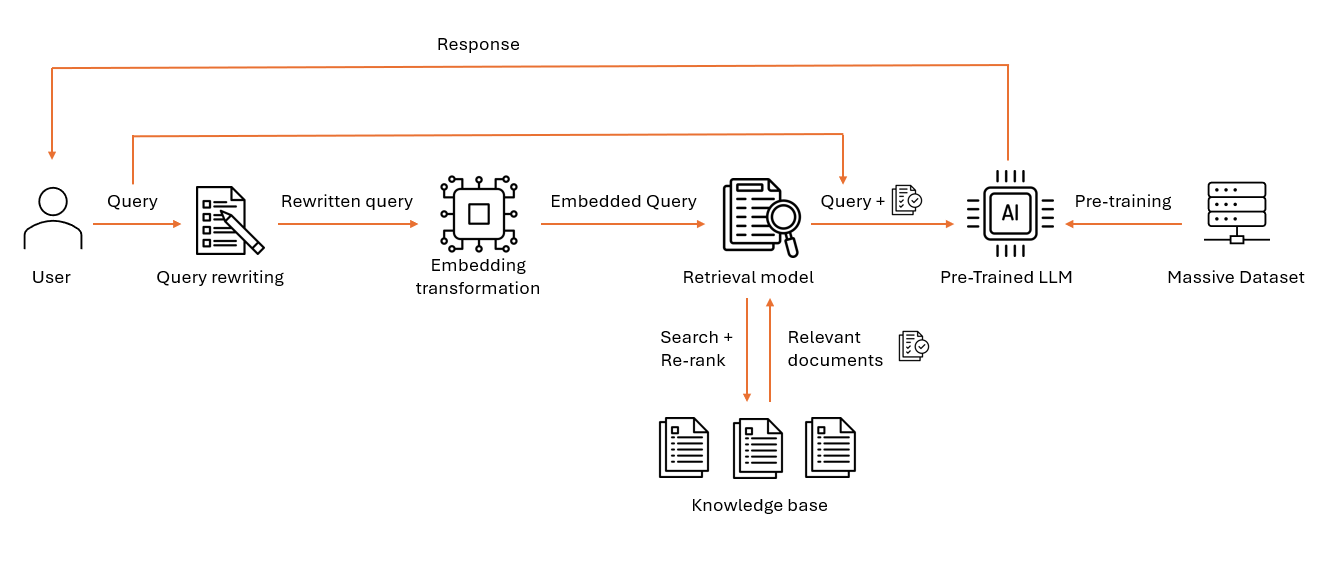
\includegraphics[scale=0.45]{Images/Preliminaries/Retrieval-Augmented Generation Process.png}
\vspace{5mm}
\caption{Retrieval-Augmented Generation Process}
\end{figure}

The RAG process is composed of two main components: the retriever and the generator. The retriever is responsible for locating and extracting relevant information from an external knowledge source, employing techniques such as keyword-based search, semantic similarity search, or neural network-based retrieval to ensure precise results. The generator then utilizes the retrieved context to produce coherent and accurate responses, ensuring the output aligns with the user's query while maintaining relevance and context. Together, these components form a robust framework for leveraging external knowledge in generative tasks.
% The retriever focuses on identifying and gathering relevant information from an external knowledge source using methods like keyword search, semantic similarity search, or neural network-based retrieval. The generator focuses on creating accurate responses based on the context retrieved from the retriever. 

% By leveraging embedding models, which convert text into high-dimensional vectors representing semantic meaning, the retriever compares the query against stored embeddings to locate the most relevant data. This ensures that the information retrieved is both contextually appropriate and content-rich, forming a solid foundation for the next phase of the process.

\section{Mô hình Ngôn ngữ Lớn và Nhỏ (LLMs \& SLMs)}

\subsection{Sự chuyển dịch từ LLMs sang SLMs}
Trong những năm gần đây, lĩnh vực Trí tuệ Nhân tạo (AI) đã chứng kiến sự bùng nổ của các Mô hình Ngôn ngữ Lớn (Large Language Models - LLMs) như GPT-4, Claude 3, hay Gemini. Các mô hình này sở hữu hàng trăm tỷ tham số (parameters), cho phép chúng thực hiện các tác vụ phức tạp với độ chính xác cao. Tuy nhiên, việc triển khai các LLMs này đòi hỏi tài nguyên tính toán khổng lồ (thường là các cụm GPU H100/A100 trong các trung tâm dữ liệu), dẫn đến chi phí vận hành cao và độ trễ mạng đáng kể.

Để giải quyết các hạn chế này, xu hướng phát triển các Mô hình Ngôn ngữ Nhỏ (Small Language Models - SLMs) đã nổi lên như một giải pháp tối ưu cho các ứng dụng biên (edge computing) và cục bộ (on-premise). Các mô hình như \textbf{Llama 3.2} (với kích thước 1B và 3B tham số) đại diện cho thế hệ SLM mới, được tối ưu hóa để cân bằng giữa hiệu năng và tài nguyên.



Ưu điểm nổi bật của việc sử dụng SLMs trong đồ án này bao gồm:
\begin{itemize}
    \item \textbf{Quyền riêng tư dữ liệu (Data Privacy):} Toàn bộ dữ liệu nhạy cảm (như thông tin cấu hình AWS, logs bảo mật) được xử lý cục bộ trên máy tính cá nhân, không bao giờ được gửi ra ngoài internet tới các máy chủ của bên thứ ba.
    \item \textbf{Hiệu quả chi phí và năng lượng:} SLMs có thể vận hành mượt mà trên các thiết bị có phần cứng hạn chế (CPU hoặc GPU laptop thông thường), giảm thiểu chi phí hạ tầng.
    \item \textbf{Khả năng tùy biến cao:} Với kích thước nhỏ gọn, SLMs dễ dàng được tinh chỉnh (fine-tune) cho các tác vụ chuyên biệt như kiểm toán bảo mật mà không tốn quá nhiều thời gian huấn luyện.
\end{itemize}

\subsection{Mô hình Ngôn ngữ Nhỏ (SLM): Meta Llama 3.2}

Để đảm bảo cân bằng giữa hiệu năng suy luận và tài nguyên hệ thống cục bộ, chúng tôi lựa chọn **Llama 3.2** (phiên bản 3 tỷ tham số - 3B) làm mô hình trí tuệ nhân tạo nòng cốt cho các Agent. Đây là dòng mô hình ngôn ngữ nhỏ (Small Language Model - SLM) thế hệ mới nhất của Meta, được phát hành vào tháng 9/2024.

Lý do lựa chọn Llama 3.2 3B cho hệ thống kiểm toán bảo mật bao gồm:

\begin{itemize}
    \item \textbf{Tối ưu hóa cho Tác vụ Agent (Agentic Capabilities):} Khác với các mô hình ngôn ngữ truyền thống chỉ mạnh về hội thoại, Llama 3.2 được tinh chỉnh (instruction-tuned) đặc biệt cho các tác vụ "Agentic Retrieval" và "Tool Use". Điều này cho phép mô hình hiểu và ra quyết định gọi các công cụ bên ngoài (như Prowler, AWS CLI) một cách chính xác hơn so với các đối thủ cùng phân khúc.
    
    \item \textbf{Hiệu suất trên Tài nguyên thấp:} Với kỹ thuật lượng tử hóa (Quantization) chuẩn \texttt{Q4\_K\_M}, mô hình chỉ chiếm khoảng \textbf{2.0GB} bộ nhớ VRAM/RAM. Điều này cho phép chạy song song nhiều Agent (Scanner, Risk Eval, Remediation) trên một máy tính cá nhân mà không gặp hiện tượng nghẽn cổ chai về phần cứng.
    
    \item \textbf{Khả năng Suy luận vượt trội:} Theo các bảng xếp hạng công nghiệp (Industry Benchmarks), phiên bản 3B này vượt trội hơn so với Google Gemma 2 (2.6B) và Microsoft Phi-3.5 mini ở các tác vụ:
    \begin{itemize}
        \item Tuân thủ chỉ thị phức tạp (Following instructions).
        \item Tóm tắt nội dung dài (Summarization) - hữu ích cho việc tạo báo cáo.
        \item Viết lại Prompt (Prompt rewriting) - hữu ích cho việc tinh chỉnh luồng suy luận CoT.
    \end{itemize}
    
    \item \textbf{Hỗ trợ đa ngôn ngữ:} Llama 3.2 hỗ trợ chính thức 8 ngôn ngữ và được huấn luyện trên tập dữ liệu rộng hơn, giúp cải thiện khả năng xử lý các báo cáo hoặc tài liệu đan xen tiếng Anh chuyên ngành và tiếng Việt.
\end{itemize}
\begin{figure}[H]
    \centering
    \includegraphics[width=0.8\textwidth]{images/llama32_benchmark_comparison.png}
    \caption{So sánh hiệu năng giữa Llama 3.2 3B với Gemma 2 2.6B và Phi-3.5 Mini trên các tác vụ quan trọng (Nguồn: Meta AI Research)}
    \label{fig:llama_benchmark}
\end{figure}

\textbf{Thông số kỹ thuật của mô hình được triển khai:}
\begin{table}[H]
\centering
\begin{tabular}{|l|l|}
\hline
\textbf{Thuộc tính} & \textbf{Giá trị} \\ \hline
Kiến trúc (Architecture) & Llama \\ \hline
Số lượng tham số & 3.21 Tỷ (3.21B) \\ \hline
Phương pháp lượng tử hóa & Q4\_K\_M (4-bit) \\ \hline
Dung lượng mô hình & $\sim$ 2.0 GB \\ \hline
Context Window & 128k token \\ \hline
License & Llama 3.2 Community License \\ \hline
\end{tabular}
\caption{Thông số kỹ thuật của Meta Llama 3.2 3B chạy trên Ollama}
\end{table}
\subsection{Lượng tử hóa}
Để triển khai các mô hình ngôn ngữ lớn (LLM) trên hạ tầng phần cứng giới hạn (Consumer Hardware), chúng tôi áp dụng kỹ thuật \textbf{Lượng tử hóa (Quantization)}. Đây là quá trình ánh xạ các tham số của mô hình từ miền giá trị có độ chính xác cao (thường là FP16 - 16-bit Floating Point) sang miền giá trị có độ chính xác thấp hơn (như INT8 hoặc INT4) nhằm giảm thiểu kích thước bộ nhớ và tăng tốc độ tính toán.

\subsubsection{Định dạng GGUF và K-Quants}

Trong đồ án này, chúng tôi sử dụng định dạng \textbf{GGUF (GPT-Generated Unified Format)}. Đây là định dạng tệp nhị phân được tối ưu hóa cho thư viện \texttt{llama.cpp}, mang lại hai lợi ích cốt lõi:

\begin{enumerate}
    \item \textbf{Memory Mapping (mmap):} GGUF cho phép hệ điều hành ánh xạ tệp mô hình trực tiếp vào bộ nhớ ảo mà không cần tải toàn bộ vào RAM ngay lập tức, giúp khởi động mô hình cực nhanh và chia sẻ bộ nhớ hiệu quả giữa CPU/GPU.
    \item \textbf{K-Quants (k-means quantization):} Llama 3.2 được lượng tử hóa theo phương pháp \texttt{Q4\_K\_M}. Khác với lượng tử hóa tuyến tính thông thường, K-Quants chia các ma trận trọng số (weights) thành các khối nhỏ (super-blocks) và sử dụng thuật toán tối ưu hóa để gán bit quan trọng cho các tham số trọng yếu (như lớp \textit{Attention}) và giảm bit ở các lớp ít quan trọng hơn (như \textit{Feed-forward}).
\end{enumerate}

\textbf{Hiệu quả thực nghiệm:}
Việc áp dụng mức lượng tử hóa \texttt{Q4\_K\_M} cho Llama 3.2 3B giúp giảm kích thước mô hình từ $\sim 6.5$ GB (FP16) xuống còn $\sim 2.0$ GB, cho phép vận hành trơn tru trên các máy tính cá nhân có RAM 8GB mà vẫn giữ được 98-99\% hiệu năng (perplexity score) so với bản gốc.
\subsection{Nền tảng Ollama và Kiến trúc suy luận cục bộ}
\textbf{Ollama} là một khung làm việc (framework) mã nguồn mở giúp đơn giản hóa việc chạy các LLM/SLM cục bộ trên macOS, Linux và Windows. Ollama đóng vai trò như một lớp trừu tượng hóa (abstraction layer), quản lý việc tải mô hình, quản lý bộ nhớ, và cung cấp giao diện API tương thích với chuẩn OpenAI.

Kiến trúc của Ollama bao gồm các thành phần chính:
\begin{itemize}
    \item \textbf{Ollama Server:} Một tiến trình nền (daemon) chịu trách nhiệm quản lý vòng đời của mô hình và xử lý các yêu cầu HTTP từ client.
    \item \textbf{Modelfile:} Một tệp cấu hình định nghĩa các tham số của mô hình, bao gồm \texttt{SYSTEM PROMPT} (lời nhắc hệ thống), nhiệt độ (temperature), và các tham số lấy mẫu khác. Đây là nơi chúng em lập trình hành vi cho từng Agent chuyên biệt (như Planning Agent, Remediation Agent).
    \item \textbf{REST API:} Cung cấp các điểm cuối (endpoints) như \texttt{/api/generate} và \texttt{/api/chat} để các ứng dụng Python có thể tương tác với mô hình một cách dễ dàng.
\end{itemize}

\subsection{Kỹ thuật Prompt Engineering và Fine-tuning}
Để tối ưu hóa hiệu suất của Llama 3.2 cho tác vụ kiểm toán bảo mật, đồ án áp dụng  kỹ thuật chính:
\begin{enumerate}
    \item \textbf{Chain-of-Thought (CoT) Prompting:} Trong kiến trúc Multi-Agent của đồ án, chúng em áp dụng CoT để khắc phục hạn chế của việc lập trình các quy tắc cứng (hardcoding). Kỹ thuật này cho phép các tác nhân (agents) thực hiện suy luận từng bước dựa trên dữ liệu đầu vào, giúp hệ thống tự động thích nghi và đưa ra các quyết định phù hợp với ngữ cảnh động thay vì tuân theo các kịch bản định sẵn.\end{enumerate}
\section{Framework LangChain}

Để xây dựng nền tảng cho các tác nhân AI (Agents), chúng em sử dụng \textbf{LangChain} - một khung làm việc (framework) mã nguồn mở giúp đơn giản hóa việc phát triển các ứng dụng dựa trên Mô hình Ngôn ngữ Lớn (LLM). LangChain đóng vai trò là framework kết nối logic lập trình với khả năng suy luận của mô hình Llama 3.2.

\subsection{Vai trò trong Kiến trúc Hệ thống}
Trong đồ án này, LangChain không chỉ đơn thuần là công cụ gọi API, mà còn đảm nhận các nhiệm vụ cốt lõi:
\begin{itemize}
    \item \textbf{Trừu tượng hóa Model (Model Abstraction):} Cung cấp giao diện thống nhất để tương tác với Ollama. Điều này cho phép hệ thống dễ dàng chuyển đổi giữa các mô hình (ví dụ: từ Llama 3.2 sang Mistral) mà không cần sửa đổi mã nguồn nghiệp vụ.
    \item \textbf{Quản lý Prompt (Prompt Engineering):} Sử dụng \texttt{PromptTemplate} để cấu trúc hóa đầu vào, kết hợp các biến động (như dữ liệu log Prowler) với các chỉ thị cố định (System Prompt).
    \item \textbf{Định dạng đầu ra (Output Parsing):} Chuyển đổi văn bản tự nhiên do LLM sinh ra thành các định dạng dữ liệu có cấu trúc (JSON, List) để các module phần mềm có thể xử lý tiếp.
\end{itemize}

\subsection{LangChain Expression Language (LCEL)}

Hệ thống được xây dựng dựa trên \textbf{LCEL} - một cú pháp khai báo (declarative) giúp kết nối các thành phần thành một chuỗi xử lý (chain) liền mạch. LCEL lấy cảm hứng từ toán tử "pipe" trong Unix, cho phép luồng dữ liệu di chuyển tuyến tính và minh bạch.

Một chuỗi xử lý điển hình trong đồ án được định nghĩa như sau:

\begin{equation}
    \text{Chain} = \text{Prompt} \: | \: \text{LLM} \: | \: \text{OutputParser}
\end{equation}

Trong đó:
\begin{itemize}
    \item \textbf{Prompt:} Nhận biến đầu vào (ví dụ: \texttt{user\_request}) và tạo ra đoạn văn bản hoàn chỉnh gửi cho mô hình.
    \item \textbf{LLM:} Thực hiện suy luận (Inference) dựa trên prompt.
    \item \textbf{OutputParser:} Trích xuất phần nội dung quan trọng từ phản hồi của LLM và loại bỏ các ký tự dư thừa.
\end{itemize}

Ví dụ mã nguồn minh họa việc áp dụng LCEL trong tác nhân \textit{Planning Agent}:

\begin{verbatim}
# Minh họa cấu trúc LCEL trong mã nguồn
prompt = PromptTemplate.from_template("Lập kế hoạch quét cho dịch vụ: {service}")
llm = ChatOllama(model="llama3.2")
parser = JsonOutputParser()

# Khởi tạo chuỗi xử lý
chain = prompt | llm | parser

# Thực thi
plan = chain.invoke({"service": "AWS S3"})
\end{verbatim}

\subsection{Tích hợp Công cụ (Tool Integration)}
LangChain cho phép mở rộng khả năng của Llama 3.2 thông qua các \textbf{Tools}. Trong hệ thống này, chúng em định nghĩa các hàm Python (như \texttt{run\_prowler\_scan}, \texttt{aws\_cli\_exec}) và bọc chúng dưới dạng LangChain Tools. Nhờ đó, Agent có thể "nhận thức" được môi trường và tác động thực tế lên hạ tầng Cloud thay vì chỉ trả lời lý thuyết suông.
\section{Framework LangGraph}

Trong khi LangChain cung cấp các khối xây dựng cơ bản (chains) hoạt động theo cơ chế đồ thị không chu trình có hướng (Directed Acyclic Graph - DAG), việc xây dựng các hệ thống tác nhân phức tạp đòi hỏi khả năng xử lý vòng lặp (loops) và duy trì trạng thái bền vững. Để giải quyết vấn đề này, chúng em sử dụng \textbf{LangGraph} - một thư viện mở rộng của LangChain chuyên dụng cho việc điều phối các ứng dụng có trạng thái (stateful) và đa tác nhân.

\subsection{Kiến trúc Đồ thị Trạng thái (StateGraph Architecture)}

LangGraph mô hình hóa luồng xử lý của ứng dụng dưới dạng một \textbf{Đồ thị Trạng thái (StateGraph)}. Khác với các chuỗi xử lý tuyến tính, kiến trúc này cho phép định nghĩa các luồng công việc có tính chu kỳ (cyclic workflows), nơi đầu ra của một bước có thể quay trở lại làm đầu vào cho bước trước đó hoặc điều hướng sang nhánh khác dựa trên logic điều kiện.

Một đồ thị trong LangGraph được định nghĩa bởi bộ ba thành phần:
\begin{equation}
    G = (S, N, E)
\end{equation}

Trong đó:
\begin{itemize}
    \item \textbf{State ($S$):} Là lược đồ dữ liệu chia sẻ (Shared Schema), đóng vai trò như bộ nhớ chung cho toàn bộ đồ thị. Tất cả các Node đều truy cập và cập nhật vào State này thay vì truyền tham số trực tiếp cho nhau.
    \item \textbf{Nodes ($N$):} Là các đơn vị xử lý logic (thường là các Agent hoặc các hàm Python). Mỗi Node nhận State hiện tại làm đầu vào, thực hiện tính toán, và trả về một bản cập nhật trạng thái (State Update).
    \item \textbf{Edges ($E$):} Quy định luồng di chuyển giữa các Nodes.
\end{itemize}

\subsection{Cơ chế Quản lý Trạng thái (State Management)}

Điểm mạnh cốt lõi của LangGraph là cơ chế quản lý trạng thái tập trung. Trong đồ án này, trạng thái hệ thống được định nghĩa bằng cấu trúc \texttt{TypedDict} của Python.

Khi một Node hoàn thành tác vụ, nó không ghi đè toàn bộ trạng thái mà trả về một phần thay đổi (delta). LangGraph sẽ tự động hợp nhất (merge) thay đổi này vào trạng thái toàn cục:
\begin{equation}
    S_{t+1} = S_t \cup \Delta S_{node}
\end{equation}
Cơ chế này đảm bảo tính toàn vẹn dữ liệu khi nhiều tác nhân cùng tham gia vào quy trình xử lý (ví dụ: \textit{Scanner Agent} cập nhật danh sách lỗi, trong khi \textit{Risk Agent} cập nhật điểm rủi ro vào cùng một State).

\subsection{Điều hướng Luồng và Vòng lặp (Control Flow \& Cycles)}

LangGraph cung cấp hai loại cạnh để điều khiển luồng đi:

\begin{enumerate}
    \item \textbf{Cạnh thường (Normal Edges):} Chuyển đổi trực tiếp từ Node A sang Node B (ví dụ: Từ \textit{Planning} $\rightarrow$ \textit{Scan}).
    \item \textbf{Cạnh điều kiện (Conditional Edges):} Sử dụng hàm logic để quyết định điểm đến tiếp theo dựa trên trạng thái hiện tại. Đây là nền tảng của mô hình "Human-in-the-loop" và khả năng tự sửa lỗi.
\end{enumerate}



Ví dụ minh họa logic cạnh điều kiện trong hệ thống:
\begin{verbatim}
# Logic định tuyến dựa trên trạng thái
def route_after_assessment(state):
    if state["risk_level"] == "CRITICAL":
        return "remediate_node"  # Chuyển sang sửa lỗi
    else:
        return "report_node"     # Chuyển sang báo cáo

workflow.add_conditional_edges("assessment", route_after_assessment)
\end{verbatim}

Nhờ LangGraph, hệ thống có thể thực hiện các quy trình phức tạp như: \textit{Quét $\rightarrow$ Đánh giá $\rightarrow$ Sửa lỗi $\rightarrow$ Quét lại (Rescan)}. Bước "Quét lại" chính là một vòng lặp (cycle) mà các chuỗi LangChain truyền thống khó thực hiện được.\
section{Hệ thống Đa tác nhân (Multi-Agent Systems)}

Hệ thống được xây dựng dựa trên mô hình Đa tác nhân (Multi-Agent System - MAS) sử dụng framework \textbf{LangChain} và \textbf{LangGraph}. Thay vì xử lý tuyến tính, hệ thống quản lý trạng thái (State) và điều phối luồng công việc giữa các tác nhân chuyên biệt dưới dạng một đồ thị có hướng (State Graph).

Hệ thống bao gồm 3 tác nhân chính phối hợp với nhau để thực hiện quy trình kiểm toán và khắc phục bảo mật:

\subsection{Cấu trúc của một Tác nhân (Agent Structure)}

Trong ngữ cảnh của đồ án, mỗi tác nhân (Agent) không phải là một thực thể trừu tượng phức tạp mà được cấu thành từ 3 thành phần cơ bản:
\begin{itemize}
    \item \textbf{Profile (Prompt):} Chỉ thị vai trò, nhiệm vụ cụ thể (ví dụ: "Bạn là chuyên gia đánh giá rủi ro...").
    \item \textbf{Tools (Công cụ):} Các hàm chức năng mà Agent có thể gọi (ví dụ: chạy Prowler scan, gọi AWS SDK để đổi cấu hình).
    \item \textbf{LLM (Brain):} Bộ não xử lý ngôn ngữ tự nhiên để quyết định xem nên dùng công cụ nào hoặc trả lời như thế nào dựa trên đầu vào.
\end{itemize}



\subsection{Các Tác nhân Chính (Core Agents)}

Hệ thống được chia nhỏ thành các tác nhân với trách nhiệm riêng biệt:

\begin{enumerate}
    \item \textbf{Planning Agent (Tác nhân lên kế hoạch):}
    \begin{itemize}
        \item \textbf{Nhiệm vụ:} Tiếp nhận yêu cầu từ người dùng và tiến hành suy nghĩ đưa ra kế hoạch phù hợp.
        \item \textbf{Đầu ra:} Danh sách các phát hiện (findings) thô từ môi trường AWS.
    \end{itemize}
    \item \textbf{Scanner Agent (Tác nhân Quét):}
    \begin{itemize}
        \item \textbf{Nhiệm vụ:} Tiếp nhận yêu cầu từ Planning Agent và thực thi các công cụ rà soát (Trong trường hợp đồ án là: Prowler).
        \item \textbf{Đầu ra:} Danh sách các phát hiện (findings) thô từ môi trường AWS.
    \end{itemize}

    \item \textbf{Risk Evaluation Agent (Tác nhân Đánh giá Rủi ro):}
    \begin{itemize}
        \item \textbf{Nhiệm vụ:} Phân tích các phát hiện từ Scanner Agent. Agent này sử dụng LLM để đối chiếu với các tiêu chuẩn bảo mật, loại bỏ cảnh báo giả (false positives) và chấm điểm mức độ nghiêm trọng.
        \item \textbf{Đầu ra:} Danh sách các lỗi đã được xác thực và phân loại (Critical, High, Medium).
    \end{itemize}

    \item \textbf{Remediation Agent (Tác nhân Khắc phục):}
    \begin{itemize}
        \item \textbf{Nhiệm vụ:} Nhận danh sách lỗi từ Risk Evaluation Agent. Dựa trên mức độ rủi ro và cấu hình cho phép, Agent sẽ lập kế hoạch và thực thi các lệnh sửa lỗi (auto-remediation) hoặc đưa ra hướng dẫn.
        \item \textbf{Đầu ra:} Báo cáo kết quả khắc phục (Success/Failed).
    \end{itemize}
\end{enumerate}

\subsection{Luồng hoạt động (Workflow & State Management)}
Chúng em sử dụng \textbf{LangGraph} để định nghĩa luồng di chuyển dữ liệu giữa các Agent, theo kiến trúc bên dưới đây. Trạng thái chung (Shared State) của hệ thống đóng vai trò như bộ nhớ chia sẻ, lưu trữ các thông tin quan trọng qua từng bước.



Quy trình xử lý được mô hình hóa đơn giản như sau:
\begin{algorithm}[H]
\caption{AWS Security Audit Workflow (LangGraph Orchestration)}
\label{alg:workflow_real}
\begin{algorithmic}[1]
\Require User Request $R$ (e.g., "Scan S3 and IAM")
\Ensure Final Report Path $P$

\State $State \leftarrow \text{InitState}(R)$

\State $State.Plan \leftarrow \Call{PlanningAgent}{R}$ \Comment{Phân tích yêu cầu}
\State $JobIDs \leftarrow \Call{ScannerAgent}{State.Plan}$
\State $State.RawFindings \leftarrow \Call{MonitorAgent}{JobIDs}$ \Comment{Đợi kết quả Prowler}

\State $Enriched \leftarrow \Call{RiskEvalAgent}{State.RawFindings}$ \Comment{Thêm ngữ cảnh rủi ro}
\State $State.Failures, NeedFix \leftarrow \Call{AssessmentAgent}{Enriched}$ \Comment{Lọc lỗi vi phạm}

\If{$NeedFix \textbf{ is } True$}
    \State $Approval \leftarrow \Call{HumanReviewNode}{State.Failures}$ \Comment{Hỏi người dùng}
    \If{$Approval \textbf{ is } Yes$}
        \State $\Call{RemediateAgent}{State.Failures}$ \Comment{Tự động sửa lỗi}
    \EndIf
\EndIf

\State $PostScanData \leftarrow \Call{RescanAgent}{}$ \Comment{Quét lại kiểm chứng}
\State $Diff \leftarrow \Call{AnalysisAgent}{State.RawFindings, PostScanData}$ \Comment{So sánh trước/sau}
\State $P \leftarrow \Call{ReportAgent}{Diff}$ \Comment{Viết Markdown}

\State \Return $P$
\end{algorithmic}
\end{algorithm}
\subsection{Cơ chế Phản hồi và Suy luận (Reasoning Loop)}

Để tránh việc hardcode (lập trình cứng) các quy tắc, các Agent sử dụng kỹ thuật \textbf{ReAct (Reasoning + Acting)}. Khi gặp một lỗi bảo mật:
\begin{enumerate}
    \item \textbf{Thought (Suy nghĩ):} Agent phân tích lỗi này thuộc dịch vụ nào (ví dụ: S3 Bucket public).
    \item \textbf{Action (Hành động):} Agent chọn công cụ tương ứng (ví dụ: \texttt{s3\_block\_public\_access}).
    \item \textbf{Observation (Quan sát):} Agent kiểm tra kết quả trả về từ công cụ để xác nhận lỗi đã được sửa hay chưa trước khi báo cáo hoàn thành.
\end{enumerate}